%% chapter12_slides.tex  -  Chapter 12: Static and Dynamic Nested Sampling for Yield Curve Model Selection
%% Bayesian Machine Learning in Quantitative Finance: Theory and Practical Applications
%% Mongwe, Mbuvha & Marwala (Springer, 2025)
%% Compile: pdflatex -interaction=nonstopmode chapter12_slides.tex  (twice)
\documentclass[aspectratio=169,10pt]{beamer}

\usetheme{Madrid}
\usecolortheme{seahorse}
\usefonttheme{professionalfonts}

%% packages
\usepackage{amsmath,amssymb,mathtools}
\usepackage{bm}
\usepackage{graphicx}
\usepackage{booktabs}
\usepackage{array}
\usepackage{listings}
\usepackage{xcolor}
\usepackage{tikz}
\usetikzlibrary{arrows.meta,positioning,shapes.geometric,fit}

\graphicspath{{figures/}}

%% listings style
\definecolor{codegray}{rgb}{0.95,0.95,0.95}
\lstdefinestyle{pycode}{
  language=Python,
  basicstyle=\ttfamily\scriptsize,
  keywordstyle=\color{blue!60!black}\bfseries,
  commentstyle=\color{green!50!black}\itshape,
  stringstyle=\color{orange!80!black},
  numbers=left,
  numberstyle=\tiny\color{gray},
  numbersep=5pt,
  frame=single,
  backgroundcolor=\color{gray!7},
  tabsize=4,
  showstringspaces=false,
  breaklines=true,
  captionpos=b,
}
\lstset{style=pycode}

%% custom colours
\definecolor{myblue}{RGB}{33,102,172}
\definecolor{myorange}{RGB}{214,96,77}
\definecolor{mylightblue}{RGB}{171,217,233}

%% footline, no navigation symbols
\setbeamertemplate{footline}[frame number]
\setbeamertemplate{navigation symbols}{}

%% macros
\newcommand{\btheta}{\bm{\theta}}
\newcommand{\bw}{\mathbf{w}}
\newcommand{\balpha}{\bm{\alpha}}
\newcommand{\bbeta}{\bm{\beta}}
\newcommand{\R}{\mathbb{R}}
\newcommand{\Exp}{\mathbb{E}}
\newcommand{\Prob}{\mathbb{P}}
\newcommand{\calN}{\mathcal{N}}
\newcommand{\D}{\mathrm{D}}

%%=============================================================================
\title[Bayesian ML in QF -- Ch.12]{Bayesian Machine Learning in Quantitative Finance}
\subtitle{Chapter 12: Nested Sampling for Yield Curve Model Selection}
\author{Based on Mongwe, Mbuvha \& Marwala}
\date{2025}

%%=============================================================================
\begin{document}

\begin{frame}
  \titlepage
\end{frame}

\begin{frame}{Chapter Outline}
  \tableofcontents
\end{frame}

%%=============================================================================
\section{12.1 Introduction}
%%=============================================================================

\begin{frame}[allowframebreaks]{12.1 Introduction: Why Compare Yield Curve Models?}

The yield curve --- the relationship between bond yield and maturity --- drives debt structuring, risk management, asset pricing and portfolio allocation. The Nelson--Siegel (1987) model and its extensions are the workhorse parametric models used by portfolio managers and central banks to summarise the whole curve with a handful of interpretable numbers.

As more and more variants of these models have appeared in the literature (Diebold--Li, Svensson, Vasicek, Hull--White, \ldots), a practical question becomes unavoidable: \emph{given several candidate models that all look reasonable, which one should we trust?} This is a \textbf{model selection} problem, and it can be tackled either in the frequentist paradigm (e.g.\ cross-validation) or in the Bayesian paradigm, via the \textbf{Bayesian evidence} (marginal likelihood).

\begin{block}{Two Different Bayesian Tasks (recap from earlier chapters)}
\begin{itemize}
  \item \textbf{Parameter estimation:} given \emph{one} model, find the plausible parameter values $\theta$ --- this is what MCMC methods such as Metropolis--Hastings and Hamiltonian Monte Carlo (HMC)/NUTS (Chapter 11) are built for.
  \item \textbf{Model selection:} given \emph{several} candidate models, compute the marginal likelihood (evidence) of the data under each model, and compare them. This is the focus of this chapter.
\end{itemize}
\end{block}

\begin{alertblock}{Why Not Just Use the Harmonic Mean Estimator?}
You may recall from the Bayesian evidence chapter that the \emph{harmonic mean estimator} approximates $Z$ using only posterior samples, but it is notoriously unstable: its variance can be infinite, and a handful of low-likelihood posterior draws can dominate and ruin the estimate. Other approaches such as Bayesian quadrature and the Laplace/Gaussian approximation (MacKay, 1992) either have high variance or perform badly when the true posterior is far from Gaussian or multi-modal. This chapter introduces a much more robust and general alternative: \textbf{nested sampling}.
\end{alertblock}

\framebreak

\begin{block}{What This Chapter Does}
\begin{enumerate}
  \item Defines several \textbf{subsets} of the Nelson--Siegel model (Models 1--7), obtained by switching individual factor loadings $\{\beta_0,\beta_1,\beta_2\}$ on or off.
  \item Introduces the \textbf{Automatic Relevance Determination Nelson--Siegel (ARD-NS)} model, which \emph{automatically} learns how relevant each factor loading is, rather than requiring the analyst to switch loadings on/off by hand.
  \item Explains the Bayesian evidence framework and \textbf{static} and \textbf{dynamic nested sampling} as ways of computing the evidence $Z$ (and, as a free by-product, the posterior).
  \item Runs numerical experiments: (a) simulated data, where the true generating model is known, to test whether the evidence framework can \emph{recover} the correct model; and (b) real US corporate-bond yield data, calibrated with the ARD-NS model via NUTS, to see which factor loadings matter most through time.
\end{enumerate}
\end{block}

\begin{exampleblock}{Headline Result (preview)}
On simulated data generated from Model 4 (level + slope only), the evidence framework correctly identifies Model 4 as the best model. On the real US corporate-bond data, the ARD-NS importances show that the \emph{medium-term (curvature) factor loading} $\beta_2$ is the main driver of the yield curve shape over the period studied (2019--2024).
\end{exampleblock}

\end{frame}

%%=============================================================================
\section{12.2 Yield Curve Models}
%%=============================================================================

\begin{frame}[allowframebreaks]{12.2.1 Subsets of the Nelson and Siegel Model}

\textbf{Intuition first.} The full Nelson--Siegel curve is a weighted sum of three ``shape'' functions of maturity $\tau$: a constant (flat) term, a term that decays quickly from 1 to 0 (a short-term effect), and a hump-shaped term that starts at 0, rises, then falls back to 0 (a medium-term effect). If we suspect that, on a given day, only some of these shapes are really needed to explain the curve, we can \emph{switch off} one or more of the corresponding coefficients ($\beta_0,\beta_1,\beta_2$) and see whether the data still supports the richer model or prefers the simpler one. That comparison is exactly what the Bayesian evidence is for.

\begin{block}{The Nelson and Siegel (1987) Yield Curve Function (Eq.~12.1)}
\[
  y_t(\tau) = \beta_0 + \beta_1\left(\frac{1-\exp(-\lambda\tau)}{\lambda\tau}\right)
  + \beta_2\left(\frac{1-\exp(-\lambda\tau)}{\lambda\tau} - \exp(-\lambda\tau)\right)
\]
\end{block}

\begin{block}{Notation}
\begin{itemize}
  \item $y_t(\tau)$ is the modelled yield at time $t$ for time-to-maturity $\tau$.
  \item $\{\beta_0,\beta_1,\beta_2,\lambda\}$ are the model parameters; $\beta_0>0$ and $\lambda>0$ must hold.
  \item $\beta_0$ has loading $1$ (never decays to 0) $\Rightarrow$ \textbf{long-term (level)} factor.
  \item $\beta_1$ has loading $\frac{1-\exp(-\lambda\tau)}{\lambda\tau}$, which starts at 1 and decays monotonically and quickly to 0 $\Rightarrow$ \textbf{short-term (slope)} factor.
  \item $\beta_2$ has loading $\frac{1-\exp(-\lambda\tau)}{\lambda\tau}-\exp(-\lambda\tau)$, which starts at 0, rises, then decays back to 0 $\Rightarrow$ \textbf{medium-term (curvature)} factor.
  \item In the Bayesian setting, the priors are Gaussian for $\beta_1,\beta_2$ and LogNormal for $\beta_0,\lambda$ (to respect the positivity constraints).
\end{itemize}
\end{block}

\framebreak

\begin{block}{Models 1--7: Subsets of the Nelson--Siegel Model (Eqs.~12.2--12.8)}
To assess the impact of each factor loading, the chapter compares seven models obtained by setting some of $\{\beta_0,\beta_1,\beta_2\}$ to zero:
\begin{center}
{\scriptsize
\begin{tabular}{clccc l}
\toprule
Model & Formula & $\beta_0$ & $\beta_1$ & $\beta_2$ & Interpretation \\
\midrule
1 & $y_t(\tau)=\beta_0$ & \checkmark & & & level only \\
2 & $y_t(\tau)=\beta_1\left(\frac{1-e^{-\lambda\tau}}{\lambda\tau}\right)$ & & \checkmark & & slope only \\
3 & $y_t(\tau)=\beta_2\left(\frac{1-e^{-\lambda\tau}}{\lambda\tau}-e^{-\lambda\tau}\right)$ & & & \checkmark & curvature only \\
4 & $y_t(\tau)=\beta_0+\beta_1(\cdots)$ & \checkmark & \checkmark & & level + slope \\
5 & $y_t(\tau)=\beta_0+\beta_2(\cdots)$ & \checkmark & & \checkmark & level + curvature \\
6 & $y_t(\tau)=\beta_1(\cdots)+\beta_2(\cdots)$ & & \checkmark & \checkmark & slope + curvature \\
7 & $y_t(\tau)=\beta_0+\beta_1(\cdots)+\beta_2(\cdots)$ & \checkmark & \checkmark & \checkmark & \textbf{full NS model} \\
\bottomrule
\end{tabular}
}
\end{center}
Model 7 is the full Nelson--Siegel model; Models 1--6 are proper subsets, each missing one or two loadings.
\end{block}

\begin{alertblock}{Why This Matters for Model Selection}
Models 1--3 use only a single factor loading, so they can only produce \emph{monotone or flat} yield curves --- they cannot reproduce a realistically shaped curve. Models 4--7 combine two or three loadings and can fit much richer shapes. The Bayesian evidence framework (Sect.~12.3) lets us rank all seven models quantitatively, automatically penalising models that are more complex than the data requires (Occam's razor).
\end{alertblock}

\end{frame}

\begin{frame}[fragile]{Python: Nelson--Siegel Loadings and the Seven Subset Models}
\begin{lstlisting}[caption={Building blocks for the seven subset Nelson-Siegel models (Eqs. 12.1-12.8)}]
import numpy as np

def ns_loadings(tau, lam):
    """Nelson-Siegel factor loadings for maturities tau and decay lam."""
    x1 = (1 - np.exp(-lam * tau)) / (lam * tau)   # short-term (slope) loading
    x2 = x1 - np.exp(-lam * tau)                  # medium-term (curvature) loading
    return x1, x2

def yield_curve(tau, beta0, beta1, beta2, lam):
    """Full Nelson-Siegel model (Model 7, Eq. 12.8)."""
    x1, x2 = ns_loadings(tau, lam)
    return beta0 + beta1 * x1 + beta2 * x2

# Models 1-7: switch individual loadings on/off (None means "fixed at 0")
MODEL_SPECS = {
    1: dict(beta0=True,  beta1=False, beta2=False),  # level only
    2: dict(beta0=False, beta1=True,  beta2=False),  # slope only
    3: dict(beta0=False, beta1=False, beta2=True),   # curvature only
    4: dict(beta0=True,  beta1=True,  beta2=False),  # level + slope
    5: dict(beta0=True,  beta1=False, beta2=True),   # level + curvature
    6: dict(beta0=False, beta1=True,  beta2=True),   # slope + curvature
    7: dict(beta0=True,  beta1=True,  beta2=True),   # full model
}

def predict(model_id, tau, params, lam):
    spec = MODEL_SPECS[model_id]
    x1, x2 = ns_loadings(tau, lam)
    y = np.zeros_like(tau, dtype=float)
    if spec["beta0"]: y = y + params["beta0"]
    if spec["beta1"]: y = y + params["beta1"] * x1
    if spec["beta2"]: y = y + params["beta2"] * x2
    return y
\end{lstlisting}
\end{frame}

\begin{frame}[allowframebreaks]{12.2.2 Automatic Relevance Determination Nelson and Siegel Model}

\textbf{Intuition first.} Instead of manually enumerating and comparing all $2^3-1$ possible subsets of $\{\beta_0,\beta_1,\beta_2\}$, can the model \emph{decide for itself}, from the data, which factor loadings actually matter? This is exactly the idea of \textbf{Automatic Relevance Determination (ARD)}: give every parameter its own individual prior variance (regularisation strength) $\alpha_i$, and let the data tell you, via posterior inference, how large or small each $\alpha_i$ should be. A large $\alpha_i$ says ``this parameter's associated factor loading is important''; a value pushed toward the prior mean (effectively shrunk to zero) says ``this loading is not needed.''

\begin{block}{ARD-NS Negative Log-Likelihood (Eq.~12.9)}
\[
  l(\D|\bw=\{\beta_0,\beta_1,\beta_3,\lambda\}) = \sum_{i}^{N}\big[y_t(\tau,\{\beta_0,\beta_1,\beta_3,\lambda\}) - y_i\big]^2
\]
\end{block}

\begin{block}{Notation}
\begin{itemize}
  \item $\D=\{\tau,y\}$ is the observed data (maturities and yields), $N$ is the number of observations.
  \item $\bw = \{\beta_0,\beta_1,\beta_3,\lambda\}$ (as labelled in the book) are the parameters to be estimated --- note this is the full three-loading (plus $\lambda$) model, i.e.\ the ARD version is built on top of Model 7.
  \item The likelihood is Gaussian, i.e.\ squared-error, matching the static nested sampling setup used later in the chapter.
\end{itemize}
\end{block}

\begin{block}{Target Posterior (Eq.~12.10)}
\[
  \ln p(\bw|\D) = l(\D|\bw) + \ln p(\bw|\alpha) + \ln q(\alpha)
\]
where $\ln p(\bw|\alpha)$ is the log of the prior on the parameters $\bw$ given the hyperparameters $\alpha$, and $\ln q(\alpha)$ is the distribution of the hyperparameters.
\end{block}

\framebreak

\begin{block}{The ARD Prior Structure}
\begin{itemize}
  \item Each parameter in $\bw$ is given a Gaussian prior with zero mean and its own standard deviation (regularisation parameter) $\alpha_i$: this is the ARD prior.
  \item The larger $\alpha_i$ is, the more important the associated parameter (factor loading) is for explaining the data.
  \item Because the loss surface induced by the ARD prior is multi-modal and non-convex, the chapter jointly samples $\bw$ \emph{and} the hyperparameters $\balpha$ together (rather than a two-stage Gibbs scheme), which produces more stable exploration.
  \item As $\bw$ is Gaussian, the $\alpha_i$'s are chosen to be \textbf{log-normally distributed} with mean 0 and variance 1, which makes the joint sampling of parameters and hyperparameters mathematically convenient.
  \item Training uses the \textbf{No-U-Turn Sampler (NUTS)} (Hoffman \& Gelman, 2011) --- the same HMC-based sampler from the previous chapter --- because it automatically tunes the step size and path length, making it easy to use without manual tuning.
\end{itemize}
\end{block}

\begin{alertblock}{Key Contrast: Fixed Subsets vs.\ ARD}
The subset models of Sect.~12.2.1 require the analyst to \emph{pre-commit} to a hard on/off pattern for each loading, then compare all patterns via evidence. The ARD-NS model instead learns a \emph{continuous, soft} importance $\alpha_i$ for each loading directly from the data in a single training run --- a loading is never literally deleted, but its effective contribution can be automatically shrunk toward negligible.
\end{alertblock}

\end{frame}

\begin{frame}[fragile]{Python: ARD Prior and NUTS Target for the ARD-NS Model}
\begin{lstlisting}[caption={Sketch of the ARD-NS log-posterior used with NUTS (Eqs. 12.9-12.10)}]
import numpy as np

def ard_ns_log_posterior(w, alpha, tau, y_obs, sigma_lik=1.0):
    """
    w     = [beta0, beta1, beta2, lam]      -- model parameters
    alpha = [a0, a1, a2, a_lam]             -- ARD hyperparameters (std devs)
    Larger alpha_i => parameter i is more "relevant" to the fit.
    """
    beta0, beta1, beta2, lam = w
    x1 = (1 - np.exp(-lam * tau)) / (lam * tau)
    x2 = x1 - np.exp(-lam * tau)
    y_pred = beta0 + beta1 * x1 + beta2 * x2

    # squared-error log-likelihood (Eq. 12.9, negated & Gaussian-normalised)
    resid = y_obs - y_pred
    log_lik = -0.5 * np.sum(resid**2) / sigma_lik**2

    # ARD prior: w_i ~ N(0, alpha_i^2)  -- larger alpha_i = less shrinkage
    log_prior_w = -0.5 * np.sum((np.array(w) / np.array(alpha))**2
                                + np.log(2 * np.pi * np.array(alpha)**2))

    # hyperprior: alpha_i ~ LogNormal(0, 1)
    log_hyperprior = -0.5 * np.sum((np.log(alpha))**2) - np.sum(np.log(alpha))

    return log_lik + log_prior_w + log_hyperprior   # Eq. 12.10

# In practice this log-posterior (and its gradient, via autodiff) is
# handed to a NUTS sampler (e.g. PyMC / NumPyro), which jointly draws
# posterior samples of w and alpha -- see Chapter 11 for the NUTS details.
\end{lstlisting}
\end{frame}

%%=============================================================================
\section{12.3 Bayesian Evidence Framework}
%%=============================================================================

\begin{frame}[allowframebreaks]{12.3 The Bayesian Evidence Framework --- Recap and Notation}

\textbf{Intuition first.} To choose between models, Bayesian inference does not stop at estimating parameters $\theta$ for a single model $M$ --- it also asks: \emph{how well does model $M$, averaged over its whole prior, explain the observed data?} That number is the evidence $Z_M$, and comparing $Z_M$ across models is a principled, built-in Occam's razor: a model with a large parameter space that only fits the data well in a tiny corner of that space earns a low evidence, even if its best-fit likelihood is very high.

\begin{block}{Bayes' Theorem for Parameters Given a Model (Eq.~12.11)}
\[
  P(\theta|\D,M) = \frac{P(\D|\theta,M)\,P(\theta|M)}{P(\D|M)}
\]
\end{block}

\begin{block}{The Evidence (Marginal Likelihood) (Eq.~12.12)}
\[
  P(\D|M) = \int_{\Omega_\theta} P(\D|\theta,M)\,P(\theta|M)\,d\theta
\]
where $P(\D|\theta,M)$ is the likelihood, $P(\theta|M)$ the prior, and the integral runs over the whole parameter domain $\Omega_\theta$ (possibly high-dimensional). This evidence \emph{naturally penalises unnecessarily complex models}: two models can share the same best-fit likelihood but very different evidence if one wastes prior mass on parameter regions that do not fit the data well.
\end{block}

\framebreak

\begin{block}{Shorthand Notation Used in this Chapter (Eq.~12.13)}
\[
  P(\theta_M) = \frac{L(\theta_M)\,\pi(\theta_M)}{Z_M}
\]
\begin{itemize}
  \item $P(\theta_M) := P(\theta|\D,M)$ is the posterior.
  \item $L(\theta_M) := P(\D|\theta,M)$ is the likelihood.
  \item $\pi(\theta_M) := P(\theta|M)$ is the prior.
  \item $Z_M := P(\D|M)$ is the evidence.
\end{itemize}
\end{block}

\begin{block}{The Bayes Factor (Eq.~12.14)}
\[
  BF := \frac{Z_{M_1}}{Z_{M_2}}\cdot\frac{\pi(M_1)}{\pi(M_2)}
\]
where $\pi(M_i)$ is the prior belief in model $i$. If all models are equally likely a priori, comparing $BF$ reduces to simply comparing $Z_{M_1}$ and $Z_{M_2}$. $BF>1$ favours $M_1$; $BF<1$ favours $M_2$.
\end{block}

\begin{alertblock}{The Practical Problem}
$Z_M$ is usually analytically intractable for realistic models --- the integral over $\Omega_\theta$ has no closed form and $\theta$ can be high-dimensional. The rest of this section introduces \textbf{nested sampling} (static and dynamic), a numerical method that computes $Z_M$ directly, with the posterior $P(\theta_M)$ falling out as a useful by-product at no extra cost.
\end{alertblock}

\end{frame}

\begin{frame}[allowframebreaks]{12.3.1 Static Nested Sampling --- The Core Trick}

\textbf{Intuition first.} The evidence integral $Z_M = \int L(\theta_M)\pi(\theta_M)\,d\theta$ is hard because $\theta$ may live in many dimensions. Nested sampling's key idea (Skilling, 2006) is to stop thinking about \emph{where in $\theta$-space} we are, and instead track only \emph{how much prior probability mass currently has likelihood above some threshold}. That single number --- called the \textbf{prior volume} $X$ --- turns the multidimensional integral into an ordinary, easy 1D integral.

\begin{block}{Re-expressing the Evidence (Eq.~12.15) and the Prior Volume $X$}
\[
  Z_m = \int_{\Omega_\theta} L(\theta_M)\,\pi(\theta_M)\,d\theta
\]
Divide the prior parameter space $\Omega_\theta$ and order it by the likelihood $L(\theta_M)$. Let $X$ denote the total enclosed prior mass, so that each unit of prior mass is $dX = \pi(\theta_M)\,d\theta$. The likelihood, viewed as a function of $X$ instead of $\theta$, is written $L(\theta_M)=L(X)$.
\end{block}

\begin{block}{The Evidence as a 1D Integral (Eq.~12.16)}
\[
  Z_m = \int_0^1 L(X)\,dX
\]
Here $X=1$ corresponds to the \emph{entire} prior (no likelihood constraint yet), and $X=0$ corresponds to the infinitesimally small region right at the peak of the likelihood. As we shrink from $X=1$ down to $X=0$, $L(X)$ increases monotonically (by construction, since we always discard the lowest-likelihood point) --- so this really is now just the area under an ordinary, monotone 1D curve, computable with e.g.\ the trapezoidal rule.
\end{block}

\framebreak

\begin{center}
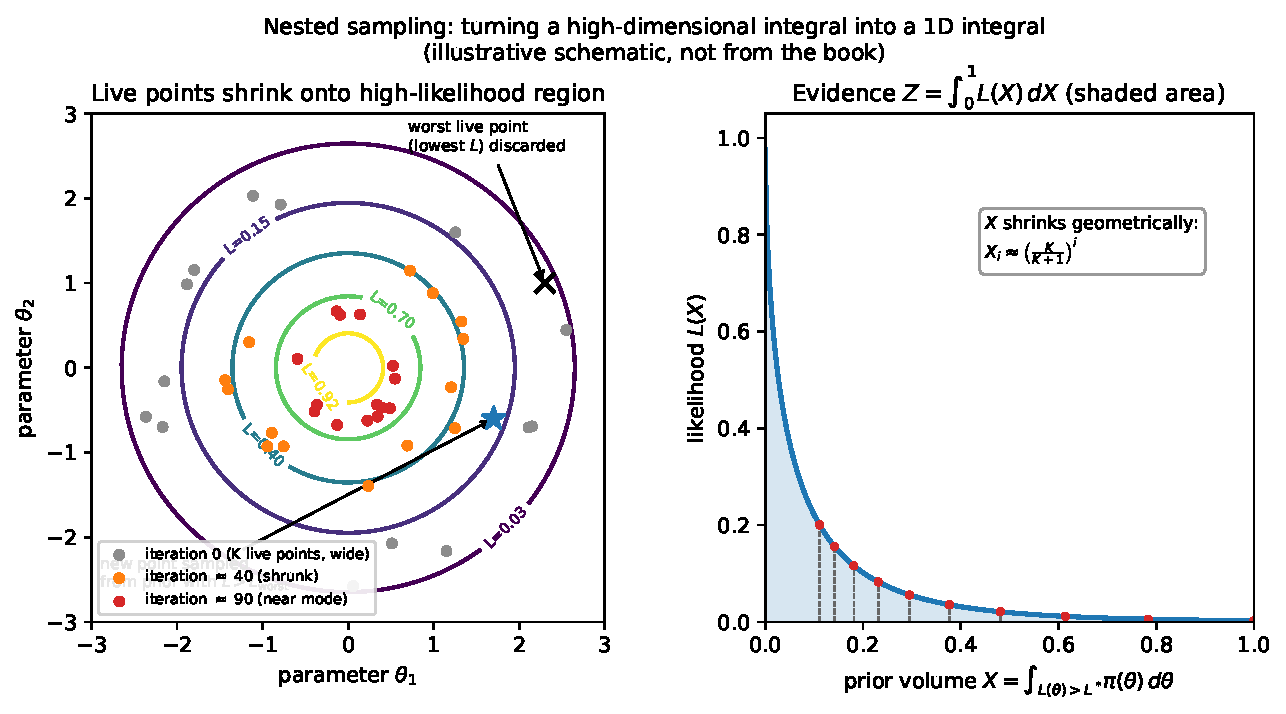
\includegraphics[width=0.92\linewidth]{ns_schematic.pdf}
\end{center}
{\small \textbf{Left:} live points (small circles/stars) shrink from the wide prior onto the high-likelihood region as the algorithm proceeds; a worst point is repeatedly discarded and replaced by a better one sampled under the current likelihood constraint. \textbf{Right:} the same process viewed in $X$-space: $L(X)$ is a monotone curve, the evidence is simply the shaded area beneath it, and the $X_i$ shrink geometrically at each iteration (illustrative schematic, not from the book).}

\end{frame}

\begin{frame}{Algorithm 12.1: Static Nested Sampling (transcribed exactly)}

\begin{block}{Algorithm 12.1: Static Nested Sampling}
\textbf{Data:} Training dataset $\{\mathbf{X}^{(i)},\mathbf{Y}^{(i)}\}$, $K$ live points \\
\textbf{Result:} Evidence $Z_m$ and posterior distribution of parameters $P(\theta_M)$

\textbf{begin}
\begin{enumerate}
  \item Sample $K$ parameter values from the prior and evaluate their likelihoods.
  \item Order the live points $K$ by their likelihoods.
  \item Select the live point that results in the lowest likelihood, and increment the evidence by some summation rule.
  \item Remove the live point with the lowest likelihood from the original $K$ live points.
  \item Replace it with a new live point sampled from the prior within the remaining prior volume. The new live point must have a higher likelihood than the discarded live point's likelihood.
  \item Repeat steps 2 to 5 until some stopping criterion is reached. This could be the desired precision on the evidence or some iteration count.
\end{enumerate}
\textbf{end}
\end{block}

\begin{alertblock}{Reading the Algorithm}
Every discard-and-replace cycle shrinks the enclosed prior volume $X$ by a known, predictable factor (in expectation, by a factor of $K/(K+1)$ for $K$ live points), and the discarded point's likelihood tells you the height $L(X)$ at that shrinkage level. Summing (discarded likelihood) $\times$ (volume shrunk) over all iterations builds up the 1D evidence integral $Z_m=\int_0^1 L(X)\,dX$ piece by piece, exactly as in Eq.~12.16.
\end{alertblock}
\end{frame}

\begin{frame}[allowframebreaks]{Toy Numeric Trace of Algorithm 12.1}

To make Algorithm 12.1 completely concrete, work through a tiny toy example \emph{by hand}. Suppose (purely for illustration) that after transforming to $X$-space the likelihood is known analytically as $L(X)=\exp(-X)$ for $X\in[0,1]$, and we use $K=5$ live points. The exact evidence is
\[
  Z = \int_0^1 e^{-X}\,dX = 1-e^{-1} \approx 0.6321.
\]
With $K=5$ live points, the expected one-step shrinkage factor is $t = K/(K+1) = 5/6 \approx 0.8333$, so $X_i \approx t^{\,i}$.

\begin{block}{Step-by-Step Trace (Steps 2--5 of Algorithm 12.1, five iterations)}
\begin{center}
{\footnotesize
\begin{tabular}{cccccc}
\toprule
Iter.\ $i$ & $X_i=(5/6)^i$ & $L_i=e^{-X_i}$ & $\Delta X_i=X_{i-1}\!-\!X_i$ & weight $\Delta X_i L_i$ & running $\hat Z$ \\
\midrule
1 & 0.8333 & 0.4346 & 0.1667 & 0.0724 & 0.0724 \\
2 & 0.6944 & 0.4994 & 0.1389 & 0.0694 & 0.1418 \\
3 & 0.5787 & 0.5606 & 0.1157 & 0.0649 & 0.2067 \\
4 & 0.4823 & 0.6175 & 0.0964 & 0.0595 & 0.2662 \\
5 & 0.4019 & 0.6690 & 0.0804 & 0.0538 & 0.3200 \\
\bottomrule
\end{tabular}
}
\end{center}
\end{block}

\begin{alertblock}{What the Numbers Show}
At each iteration the worst live point (lowest likelihood) is discarded, the prior volume shrinks from $X_{i-1}$ to $X_i$, and we add the rectangle of width $\Delta X_i$ and height $L_i$ to the running evidence estimate $\hat Z$ (step 3 of Algorithm 12.1). After only 5 iterations we have captured $0.3200$ of the true value $0.6321$ --- roughly half. This is expected: with only $K=5$ live points the volume shrinks slowly, and the algorithm must keep discarding and replacing points (step 6, ``repeat until some stopping criterion'') for many more iterations before $X$ becomes small enough that the remaining, unexplored volume contributes negligibly to $Z$. A real run would continue for on the order of $K\ln(1/X_{\text{final}})$ iterations.
\end{alertblock}

\end{frame}

\begin{frame}[fragile]{Python: A From-Scratch Static Nested Sampler}
\begin{lstlisting}[caption={Toy static nested sampler implementing Algorithm 12.1 literally}]
import numpy as np

def static_nested_sampling(log_likelihood, bounds, n_live=50, n_iter=500):
    """
    Algorithm 12.1, steps 1-6, using rejection sampling for step 5
    (adequate for low-dimensional toy problems only).
    """
    rng = np.random.default_rng(0)
    ndim = len(bounds)
    lo = np.array([b[0] for b in bounds]); hi = np.array([b[1] for b in bounds])
    sample_prior = lambda n: lo + rng.uniform(size=(n, ndim)) * (hi - lo)

    # --- Step 1: sample K live points from the prior, evaluate likelihoods
    live_theta = sample_prior(n_live)
    live_logl = np.array([log_likelihood(t) for t in live_theta])

    logZ, logX_prev = -np.inf, 0.0             # ln Z, ln X_0 = ln(1)
    t = n_live / (n_live + 1.0)                  # expected shrink factor
    for i in range(1, n_iter + 1):
        # --- Step 2: order live points by likelihood (argmin suffices)
        # --- Step 3: select the worst, increment the evidence
        worst = np.argmin(live_logl)
        logl_worst = live_logl[worst]
        logX_i = logX_prev + np.log(t)
        dX = np.exp(logX_prev) - np.exp(logX_i)
        logZ = np.logaddexp(logZ, np.log(dX) + logl_worst)

        # --- Step 4 & 5: remove worst, replace via constrained prior sampling
        while True:
            cand = sample_prior(1)[0]
            cand_logl = log_likelihood(cand)
            if cand_logl > logl_worst:            # must have higher likelihood
                break
        live_theta[worst], live_logl[worst] = cand, cand_logl
        logX_prev = logX_i
        # --- Step 6: repeat until stopping criterion (here: n_iter reached)

    # remaining live points' share of the leftover volume
    logZ = np.logaddexp(logZ, logX_prev + np.mean(live_logl))
    return logZ
\end{lstlisting}
\end{frame}

\begin{frame}{From-Scratch Toy Nested Sampler in Action}

\begin{center}
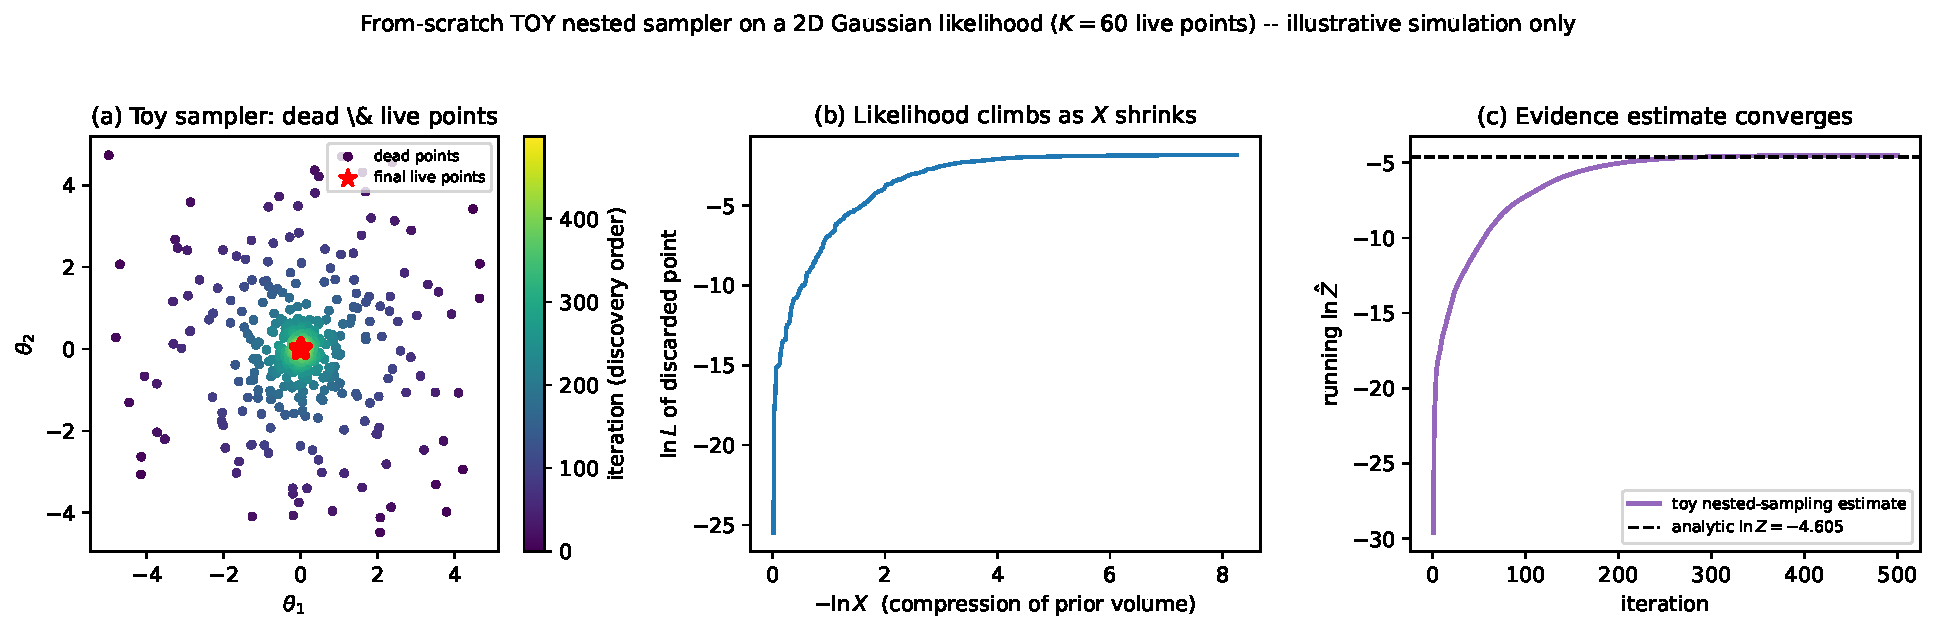
\includegraphics[width=0.98\linewidth]{toy_ns_run.pdf}
\end{center}
{\small The Python sampler on the previous slide run on a toy 2D Gaussian likelihood with $K=60$ live points. \textbf{(a)} Dead points (coloured by discovery order) spiral in on the mode; the final live points (red stars) cluster tightly around it. \textbf{(b)} The likelihood of the discarded point rises steadily as $-\ln X$ (compression of the prior volume) increases. \textbf{(c)} The running evidence estimate climbs and converges to the analytic value $\ln Z \approx -4.605$ (illustrative toy simulation).}
\end{frame}

\begin{frame}[allowframebreaks]{12.3.2 Dynamic Nested Sampling}

\textbf{Intuition first.} Static nested sampling keeps the number of live points $K$ \emph{fixed} for the whole run. But not every part of the run is equally important: early iterations (while $X$ is still close to 1) mostly just explore the bulk of the prior, while the interesting action --- where the likelihood rises steeply and most of the posterior mass concentrates --- happens in a comparatively narrow range of $X$. Static nested sampling spends the same computational effort everywhere, which is wasteful. \textbf{Dynamic nested sampling} fixes this by \emph{adaptively varying} $K$: it spends few live points where they add little information, and many live points exactly where the posterior mass (or the tails, if better tail resolution is needed) actually is.

\begin{block}{How Dynamic Nested Sampling Works (Higson et al., 2019)}
\begin{enumerate}
  \item The distribution of posterior mass as a function of likelihood is not known ahead of time, so we first approximate it with a cheap \textbf{static} nested-sampling run using a small, constant number of live points $K$.
  \item From this first pass, the algorithm iteratively determines the \emph{range of likelihoods} where adding more live points will most increase calculation accuracy.
  \item An additional \textbf{thread} (or batch) of live points is run specifically over that likelihood range.
  \item To reduce the number of times the sampler must be restarted, several threads/batches can be created at once if needed.
  \item When the batch size is small relative to the overall run, using batches larger than one has minimal effect on the efficiency gains.
\end{enumerate}
\end{block}

\framebreak

\begin{alertblock}{Static vs.\ Dynamic: Key Contrast}
\begin{itemize}
  \item \textbf{Static NS:} number of live points $K$ is \emph{constant} throughout the run.
  \item \textbf{Dynamic NS:} $K$ is \emph{continually varied} to maximise computation accuracy for a given number of posterior samples, subject to practical limits.
  \item Higson et al.\ (2019) show empirically that dynamic nested sampling \textbf{significantly improves calculation accuracy} versus static nested sampling using the \emph{same} number of samples, and that \textbf{both} evidence accuracy and posterior-estimation accuracy can be improved \emph{simultaneously}.
  \item Unlike static nested sampling, running the dynamic algorithm for \emph{longer} reliably yields \emph{more accurate} results.
\end{itemize}
\end{alertblock}

\begin{center}
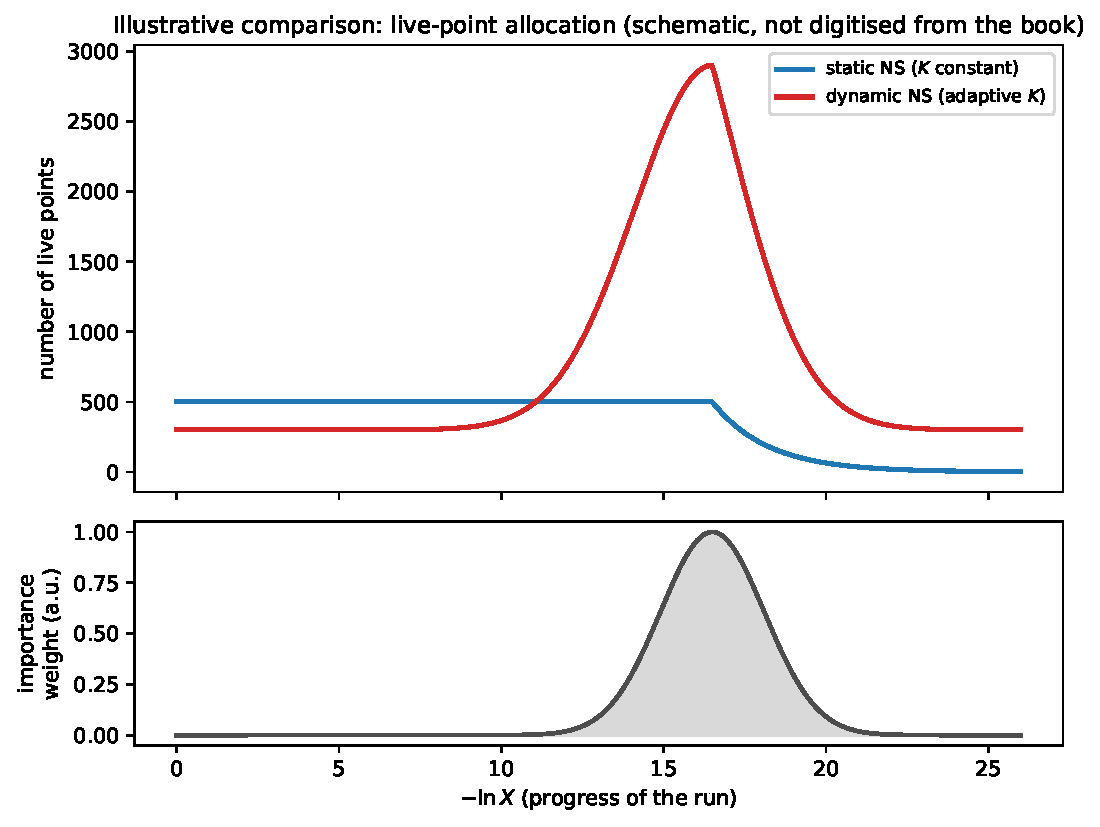
\includegraphics[width=0.72\linewidth]{static_vs_dynamic.pdf}
\end{center}
{\small Illustrative comparison (schematic shapes, not digitised from the book) of live-point allocation: static NS holds $K$ constant then runs out; dynamic NS starts with a small exploratory $K$, then concentrates additional live points precisely where the importance weight (bottom panel) --- i.e.\ the posterior mass --- peaks.}

\end{frame}

\begin{frame}[fragile]{Python: Static vs.\ Dynamic Nested Sampling with \texttt{dynesty}}
\begin{lstlisting}[caption={Book's actual tool: the dynesty package (Speagle, 2020), default settings}]
import dynesty
import numpy as np

ndim = 3  # e.g. beta0, beta1, beta2 for Model 7, lambda fixed

def loglike(theta):
    beta0, beta1, beta2 = theta
    pred = beta0 + beta1 * x1_loading + beta2 * x2_loading   # NS loadings
    resid = y_obs - pred
    return -0.5 * np.sum(resid**2) / sigma**2

def prior_transform(u):
    # map unit cube u in [0,1]^ndim to the actual prior ranges
    return -0.1 + 0.2 * u   # e.g. Uniform(-0.1, 0.1) per parameter

# --- Static nested sampling (Algorithm 12.1): K live points, fixed
sampler_static = dynesty.NestedSampler(loglike, prior_transform, ndim,
                                       nlive=500)
sampler_static.run_nested()
logZ_static = sampler_static.results.logz[-1]

# --- Dynamic nested sampling (Sect. 12.3.2): K adaptively varied
sampler_dynamic = dynesty.DynamicNestedSampler(loglike, prior_transform, ndim)
sampler_dynamic.run_nested()   # adaptively allocates live points/threads
logZ_dynamic = sampler_dynamic.results.logz[-1]

print(f"log-evidence (static)  = {logZ_static:.3f}")
print(f"log-evidence (dynamic) = {logZ_dynamic:.3f}")
\end{lstlisting}
\end{frame}

%%=============================================================================
\section{Toy Running Example: Comparing Two Subset Models}
%%=============================================================================

\begin{frame}[allowframebreaks]{Toy Running Example: Level+Slope vs.\ Level+Slope+Curvature}

\begin{alertblock}{This Is an Illustrative Toy Example, Not the Book's Result}
To build intuition before looking at the book's own numerical experiments (Sect.~12.4--12.5), here is a small \emph{self-contained} example, computed from scratch with the toy nested sampler above, comparing two Nelson--Siegel-style subset models on \emph{synthetic} data generated for this lecture only.
\end{alertblock}

\begin{block}{Setup}
\begin{itemize}
  \item Synthetic yield curve at $\tau \in \{0.25,0.5,1,2,3,5,7,10,20,30\}$ years, generated from the \emph{full} (level+slope+curvature) model with $\lambda=0.7$, $\beta_0=0.035$, $\beta_1=-0.022$, $\beta_2=0.018$, plus small Gaussian observation noise ($\sigma=0.0006$).
  \item \textbf{Model A} (toy analogue of the book's Model 4): level + slope only, i.e.\ $\beta_2$ fixed at 0.
  \item \textbf{Model B} (toy analogue of the book's Model 7): level + slope + curvature, the full model.
  \item Both models share a $\mathrm{Uniform}(-0.1,0.1)$ prior on each free $\beta$; $\lambda$ is held fixed at its true value in both models to keep the toy example simple.
  \item Evidence for each model is computed with the from-scratch toy static nested sampler shown earlier ($K=80$ live points).
\end{itemize}
\end{block}

\framebreak

\begin{center}
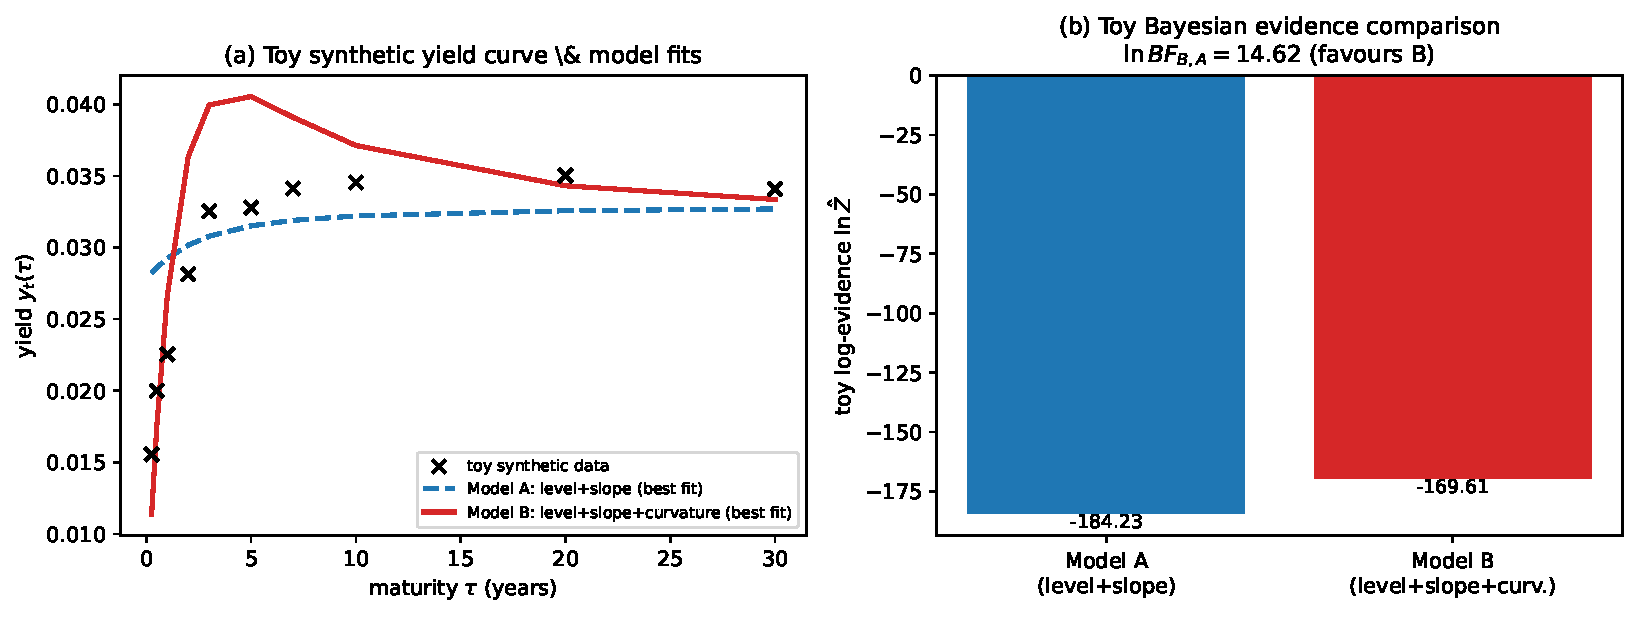
\includegraphics[width=0.95\linewidth]{toy_ns_model_comparison.pdf}
\end{center}
{\small \textbf{(a)} Toy synthetic data (crosses) together with the best-fit curves of Model A (dashed blue) and Model B (solid red). Because the data was generated with genuine curvature, Model A visibly cannot track the hump in the middle of the curve. \textbf{(b)} Toy log-evidence for each model, computed by the from-scratch sampler.}

\begin{exampleblock}{Actual Numbers from This Toy Run}
\[
  \ln \hat Z_A = -184.23, \qquad \ln \hat Z_B = -169.61, \qquad
  \ln BF_{B,A} = \ln\hat Z_B - \ln\hat Z_A = 14.62
\]
Since $\ln BF_{B,A} \gg 0$ (equivalently $BF_{B,A}=e^{14.62}\approx 2.2\times10^{6}$), the evidence \textbf{overwhelmingly favours Model B}. This is the correct conclusion: the synthetic data really was generated with a non-zero curvature term, so the extra parameter $\beta_2$ in Model B is earning its keep --- the evidence framework rewards the added complexity here \emph{because} it is genuinely needed, rather than penalising it blindly.
\end{exampleblock}

\end{frame}

%%=============================================================================
\section{12.4 Numerical Experiments}
%%=============================================================================

\begin{frame}[allowframebreaks]{12.4.1 Experiment Setup and Data Description}

\begin{block}{Two Datasets, Two Different Purposes}
\begin{itemize}
  \item \textbf{Simulated data (for model selection):} generated from Model 4 (level + slope) with known parameters $\{\beta_0=0.04,\ \beta_1=-0.05,\ \lambda=1.3\}$. Because the true generating model is known, this lets us check whether the Bayesian evidence framework can \emph{correctly identify} the model that produced the data.
  \item \textbf{Real-world data (for factor-loading analysis):} the time series of corporate bond yield curves from the US treasury/corporate market, from 1 January 2019 to 31 May 2024.
\end{itemize}
\end{block}

\begin{block}{The Experimental Pipeline}
\begin{enumerate}
  \item Calibrate \textbf{all seven} subset models (Models 1--7) to the \emph{simulated} data using \textbf{both} static and dynamic nested sampling.
  \item Perform model comparison via the Bayesian evidence metric (log $Z_m$ for each model).
  \item Calibrate the \textbf{ARD-NS} model to the \emph{real-world} data using NUTS.
  \item Analyse the resulting factor-loading importances through time.
\end{enumerate}
\end{block}

\framebreak

\begin{block}{12.4.2 Performance Metrics}
Predictive performance on unseen data is evaluated using:
\begin{itemize}
  \item \textbf{MSE} (Mean Square Error)
  \item \textbf{MAE} (Mean Absolute Error)
  \item \textbf{$R^2$} (coefficient of determination)
  \item \textbf{MAPE} (Mean Percentage Error)
\end{itemize}
\end{block}

\begin{block}{Sampler Settings}
\begin{itemize}
  \item \textbf{NUTS (for ARD-NS):} pre-conditioning matrix $\mathbf{M}=\mathbf{I}$ (the common default in practice); 5 chains of 2000 samples each, with a burn-in of 1000 samples --- sufficient for convergence on all the datasets considered.
  \item \textbf{Static and dynamic nested sampling:} implemented using the \texttt{dynesty} Python package (Speagle, 2020) with its \textbf{default settings}.
\end{itemize}
\end{block}

\end{frame}

%%=============================================================================
\section{12.5 Results and Discussions}
%%=============================================================================

\begin{frame}[allowframebreaks]{12.5 Results: Log Evidence Recovers the True Model}

\begin{block}{Table 12.1: Log Evidence on Simulated Data (True Model = Model 4)}
\begin{center}
{\scriptsize
\begin{tabular}{lcc}
\toprule
Model & Static nested sampling & Dynamic nested sampling \\
\midrule
Model 1 & $-91.951 \pm 0.133$ & $-91.929 \pm 0.076$ \\
Model 2 & $-106.615 \pm 0.222$ & $-106.559 \pm 0.158$ \\
Model 3 & $-106.250 \pm 0.219$ & $-106.612 \pm 0.152$ \\
\textbf{Model 4} & $\mathbf{-23.655 \pm 0.172}$ & $\mathbf{-23.800 \pm 0.110}$ \\
Model 5 & $-25.416 \pm 0.176$ & $-25.055 \pm 0.110$ \\
Model 6 & $-25.512 \pm 0.177$ & $-25.402 \pm 0.107$ \\
Model 7 & $-26.782 \pm 0.192$ & $-26.852 \pm 0.119$ \\
\bottomrule
\end{tabular}
}
\end{center}
\end{block}

\begin{alertblock}{Reading Table 12.1}
Static and dynamic nested sampling produce \emph{very similar} log-evidence values for every model --- reassuring agreement between the two algorithms. \textbf{Model 4 has the highest log evidence by a wide margin}, correctly identifying it as the model that generated the data. Models 1--3 (single-loading models) are the worst-ranked: they can only produce constant or monotone curves and cannot reproduce the true shape. Models 5, 6, 7 (two or three loadings, but not exactly matching the true generator) are the next-best group --- they can fit the data reasonably well but are \emph{penalised by the evidence for their unnecessary extra complexity} relative to Model 4.
\end{alertblock}

\framebreak

\begin{block}{Predictive Performance Tells a More Nuanced Story (Tables 12.2--12.3)}
On unseen simulated data, Model 4 achieves the best predictive performance under \emph{dynamic} nested sampling calibration (e.g.\ $R^2=0.999992$, MSE $=1.38\times10^{-9}$), with Model 7 a close second. Under \emph{static} nested sampling calibration, the ranking flips slightly: Model 7 gives marginally better predictive metrics, with Model 4 second. Models 1, 2, 3 perform poorly (even negative $R^2$), and Model 6 is a clear outlier with very poor fit.
\end{block}

\begin{exampleblock}{The Key Tension: Evidence vs.\ Raw Predictive Fit}
Model 7 (the full model) can match Model 4's predictive accuracy almost exactly --- unsurprising, since Model 7 contains Model 4 as a special case ($\beta_2=0$). But Model 7 has \emph{one extra free parameter}, and the evidence metric penalises this extra flexibility unless the data actually needs it. This is Occam's razor in action: near-identical predictive performance, but the evidence still prefers the more parsimonious, correctly-specified model.
\end{exampleblock}

\framebreak

\begin{block}{Factor Loading Importances Through Time (ARD-NS on Real Data)}
Training the ARD-NS model on the real US corporate bond yield time series (2019--2024) via NUTS gives, for each day, the relative importance of the short-term ($\beta_1$), medium-term ($\beta_2$), and long-term ($\beta_0$) loadings (the $\lambda$ parameter is excluded from this particular importance analysis).
\end{block}

\begin{alertblock}{Key Finding}
The \textbf{medium-term (curvature) loading $\beta_2$} is the main driver of the yield curve shape over the period studied, \textbf{followed by the short-term (slope) loading $\beta_1$}. Critically, the relative importance of each factor \emph{varies noticeably over time} --- this time-variation suggests that models which explicitly capture the temporal dynamics of the factor loadings (e.g.\ the dynamic Nelson--Siegel model of Diebold, Li \& Yue, 2008) could be a natural complementary extension for capturing yield curve dynamics through time.
\end{alertblock}

\end{frame}

%%=============================================================================
\section{12.6 Conclusion}
%%=============================================================================

\begin{frame}[allowframebreaks]{12.6 Conclusion}

\begin{block}{What This Chapter Achieved}
\begin{enumerate}
  \item Introduced \textbf{static} and \textbf{dynamic nested sampling} as ways to compute the Bayesian evidence for yield curve model selection --- a first-in-literature application to comparing subset Nelson--Siegel models.
  \item Showed, on simulated data with a known generating model, that the evidence framework \textbf{correctly identifies} the true underlying model (Model 4).
  \item Introduced the \textbf{Automatic Relevance Determination Nelson--Siegel (ARD-NS)} model, trained with NUTS, which \textbf{automatically ranks} which factor loadings (short-term, medium-term, long-term) are most relevant to a given yield curve.
  \item On real US corporate bond data (2019--2024), found that the \textbf{medium-term (curvature)} factor loading is the dominant driver of the yield curve shape, and that this relative importance \textbf{changes through time}.
\end{enumerate}
\end{block}

\begin{block}{Where This Framework Can Be Extended}
\begin{itemize}
  \item To other yield curve models beyond the Nelson--Siegel family.
  \item To other evidence-calculation methods, such as those based on normalizing flows.
  \item By combining with dynamic (time-varying) Nelson--Siegel formulations to explicitly capture how factor-loading importance evolves through time.
\end{itemize}
\end{block}

\begin{exampleblock}{Looking Ahead}
The next chapter introduces the \emph{Bayesian investment analyst} framework, which predicts directional stock movements while automatically highlighting which input features are most relevant --- a direct conceptual descendant of the automatic relevance determination idea developed here.
\end{exampleblock}

\end{frame}

\end{document}
